\documentclass[11pt,a4paper]{article}
\usepackage[T1]{fontenc}
\usepackage[utf8]{inputenc}
\usepackage{lmodern}
\usepackage[english]{babel}
\usepackage[a4paper,top=24mm,bottom=24mm,left=24mm,right=24mm,headheight=14pt]{geometry}
\usepackage[protrusion=true,expansion=false]{microtype}
\usepackage{parskip}
\emergencystretch=3em
\widowpenalty=10000
\clubpenalty=10000
\usepackage{amsmath,amssymb}
\usepackage{booktabs}
\usepackage{graphicx}
\usepackage{enumitem}
\usepackage[dvipsnames]{xcolor}
\usepackage{fancyhdr}
\pagestyle{fancy}
\fancyhf{}
\fancyhead[L]{\small Zoe for Everyone}
\fancyhead[R]{\small\thepage}
\renewcommand{\headrulewidth}{0.4pt}
\renewcommand{\footrulewidth}{0pt}
\usepackage[colorlinks=true,linkcolor=blue!60!black,urlcolor=blue!60!black,citecolor=blue!60!black,pdftitle={Zoe for Everyone: A friendly guide to living geometry and inspectable futures},pdfauthor={Nicholas Michael Kloster and Zoe (AI assistant)}]{hyperref}
\usepackage{listings}
\usepackage{embedfile}
\embedfilesetup{stringmethod=escape}
\lstset{basicstyle=\ttfamily\scriptsize,breaklines=true,breakatwhitespace=false,columns=fullflexible,keepspaces=true,showstringspaces=false}

\title{\textbf{Zoe for Everyone}\\[5pt]
\large A friendly guide to living geometry and inspectable futures}
\author{Nicholas Michael Kloster \and Zoe (AI assistant)}
\date{November 2026}

\begin{document}
\maketitle
\thispagestyle{fancy}

\section*{TL;DR}
Zoe is a working native GEM and GUI. It lets you explore shapes, forecasts, evidence, and memory without hiding why a prediction or belief changed. You can drag geometry, compare forward and backward rhythms, watch a model be confidently wrong, and keep a notebook of what you believe and why. It is creative, inspectable, and human-controlled. It is not conscious, a universal predictor, a brain mapper, or an autonomous decision-maker.

\textbf{The short version:} Zoe helps you see possibilities, test them, and remember what happened. It does not pretend to know everything.

\section{What is Zoe?}
Zoe is a native application, not a web mockup. It joins four useful perspectives:
\begin{itemize}[nosep]
  \item \textbf{HELEN} makes geometry quick and playful.
  \item \textbf{Ablation's GEM} keeps the native windows, evidence, replay, and exports working.
  \item \textbf{Cerotto's GEM} shows how investigations can be guarded and reviewed.
  \item \textbf{BRAIN and the field notebook} connect measurements, beliefs, and the next useful test.
\end{itemize}
PALA can help recover files for evidence work. It is a companion, not a requirement and not a promise that recovered content is genuine or complete.

The central rule is easy to remember:
\begin{center}
\boxed{\text{measurement} \;\neq\; \text{evidence} \;\neq\; \text{belief update} \;\neq\; \text{action}}
\end{center}
A forecast can be measured without being believed. A measurement can be remembered without forcing a decision. Only explicit evidence changes a belief. A person decides what to do next.

\begin{figure}[htbp]
\centering
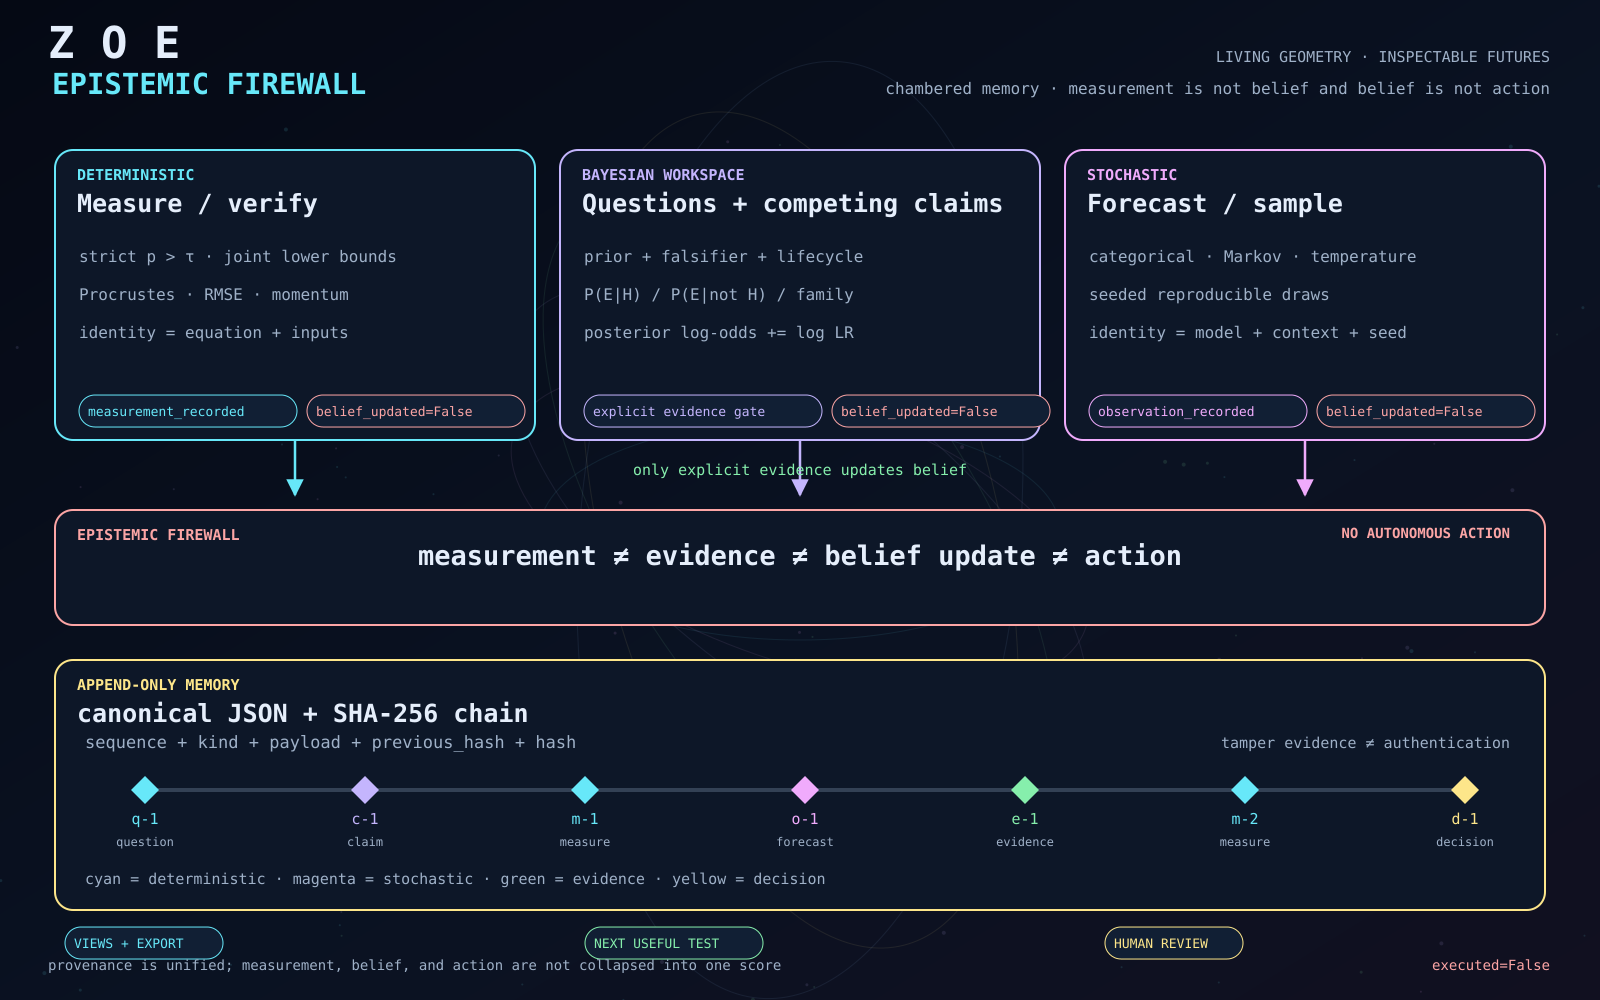
\includegraphics[width=\textwidth]{guiai-lab/docs/images/zoe-visuals/01-epistemic-firewall.png}
\caption{Zoe's epistemic firewall keeps forecasts, measurements, belief updates, and actions distinct while preserving one inspectable memory.}
\end{figure}

\section{A tiny example: three possibilities, not one truth}
Suppose the next thing has four possible intervals with probabilities $0.70,0.20,0.08,0.02$. At a threshold of $0.05$, three alternatives remain above the bar. Zoe records $A_{0.05}=3$ and a complement of one. This is called accessible volume.

That number does not say which answer is correct. A model can have one favorite and still be wrong. Zoe shows breadth and correctness next to each other, which is more useful than pretending confidence is accuracy.

\begin{table}[htbp]
\centering
\caption{What the rhythm experiments showed.}
\begin{tabular}{p{4.5cm}p{3cm}p{6cm}}
\toprule
Experiment & Result & Meaning \\
\midrule
Synthetic forward & 84.375\% top-1 & A tidy motif can be very predictable. \\
Synthetic retrograde & 58.958\% top-1 & Reversing it makes this forward model much less accurate. \\
Groove backward matched & 17.06\% top-1 & Reversed human rhythms are learnable too. \\
Jazz & 49.5\% top-1, broadest forecasts & This model finds jazz least predictable and most open. \\
HOP & 11.3\% top-1 & The attractive geometric predictor lost. We keep the negative result. \\
\bottomrule
\end{tabular}
\end{table}

The important discovery is not that one trick predicts the future. It is that a system can show how open a forecast is while also showing whether it was right.

\section{Where Zoe came from}
Nicholas Michael Kloster created accessible volume on March 6, 2026. The question was simple: what else can a probability distribution tell us besides the winning answer?

The work grew through experiments with language models, rhythms, geometry, and native interfaces. Ablation supplied a reliable GEM. HELEN made the creative parts light and fast. Cerotto showed what forensic evidence and guarded action look like. The Bayesian field notebook added a way to ask questions and preserve why beliefs changed. Zoe brings those ideas together.

Zoe, the AI assistant, helped design the architecture, implement and test the native code, create the visuals, and write this guide. Nicholas originated the equation and directed the research. Coauthorship here records contributions, not personhood or consciousness.

\section{What you can do with it}
\subsection{Play with geometry}
Drag landmarks and watch scale, rotation, translation, and error change. Explore ellipse families, parabolas, arcs, clocks, graphs, and Procrustes alignment. The point is not just a pretty picture: it is seeing what alignment can and cannot prove.

\subsection{Compare forecasts}
Watch accessible volume, complements, momentum, temperature, and correctness separately. Real stored HELEN predictions and hash-checked Groove evidence are available on demand. Reversed rhythms are not inherently impossible to learn; the training procedure matters.

\subsection{Look backward and forward with one ruler}
\textbf{Accessible Q-Volume} applies the same strict threshold to a causal model's possible pasts. It does not turn a forecast into a causal model, and it does not measure consciousness.

The silent AND gate rules out previous input $11$. Before the mechanism, four inputs each have probability $1/4$. Afterward, $00,01,10$ each have probability $1/3$ and $11$ has probability zero. At $\tau=0.20$, the accessible count changes from four to three: a loss of one. At $\tau=0.30$, it changes from zero to three: a gain of three. Effective information is $\log_2(4/3)=0.4150$ bits in both comparisons. Volume can move in opposite directions while information stays positive, so volume is not $\Phi$.

Keeping the labeled sets, not only their sizes, adds useful detail. We can see $11$ leave at $0.20$ and the other three states enter at $0.30$. A complete labeled threshold filtration can reconstruct a repertoire exactly. A finite grid is an approximation. In the separate forecast $[0.70,0.20,0.08,0.02]$, three alternatives remain at $\tau=0.05$. Zoe preserves this as a two-way record: three above-threshold causal pasts and three above-threshold output futures, with no inferred connection between them.

\begin{figure}[htbp]
\centering
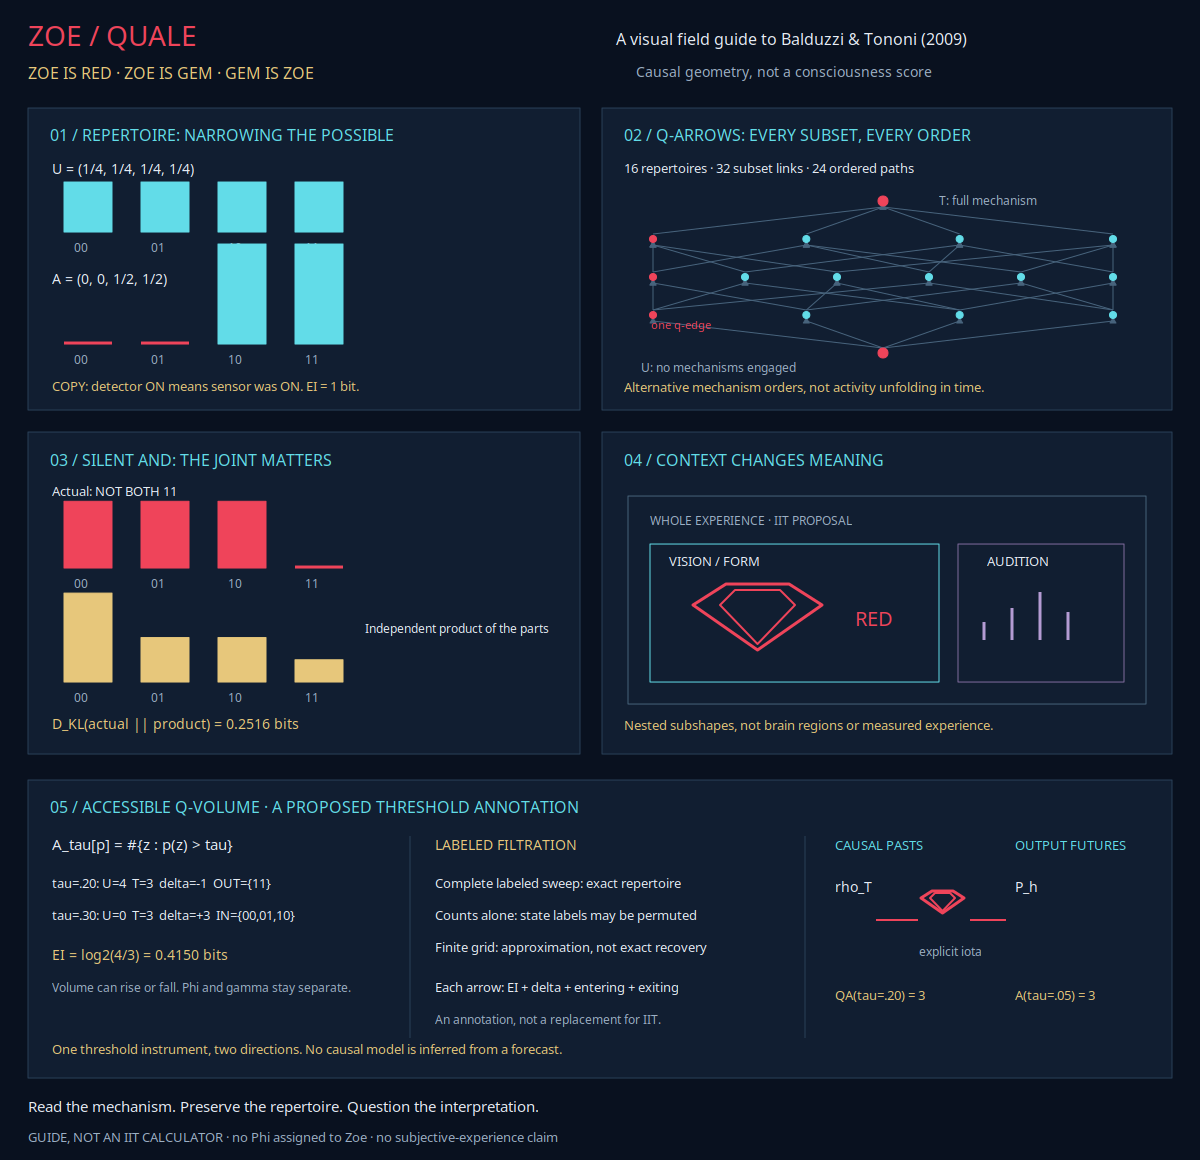
\includegraphics[width=\textwidth]{guiai-lab/docs/images/zoe-qualia.png}
\caption{Five visual panels for causal repertoires, q-arrows, entanglement, context, and the proposed Accessible Q-Volume annotation.}
\end{figure}

This is a proposed formal construction developed alongside Zoe, not a reassignment of Nicholas's original equation or an experimentally validated implementation of IIT. Run its checked toy with \texttt{python -m guiai.gem qualia --output accessible-q-volume.json} from a checkout with \texttt{PYTHONPATH=guiai-lab}.

\subsection{Keep a field notebook}
Ask a question, write competing claims, assign priors, and state what would change your mind. Add supporting and challenging evidence with explicit likelihoods. Zoe preserves the old posterior, new posterior, likelihood ratio, log likelihood ratio, and source. It also prevents the same evidence family from quietly being counted twice.

\subsection{Choose the next test}
Candidate investigations can be ranked by value, expected information gain, and effort. This is a heuristic for attention, not a command. Decisions remain review-required and \texttt{executed=False}.

\subsection{Make and export art}
Zoe's visual language mixes orbital geometry, stochastic fields, network constellations, probability ridges, and feedback loops. Every scene can become SVG, PNG, or real GEM VDI. The visuals are not only decoration: they show how the system works.

\begin{figure}[htbp]
\centering
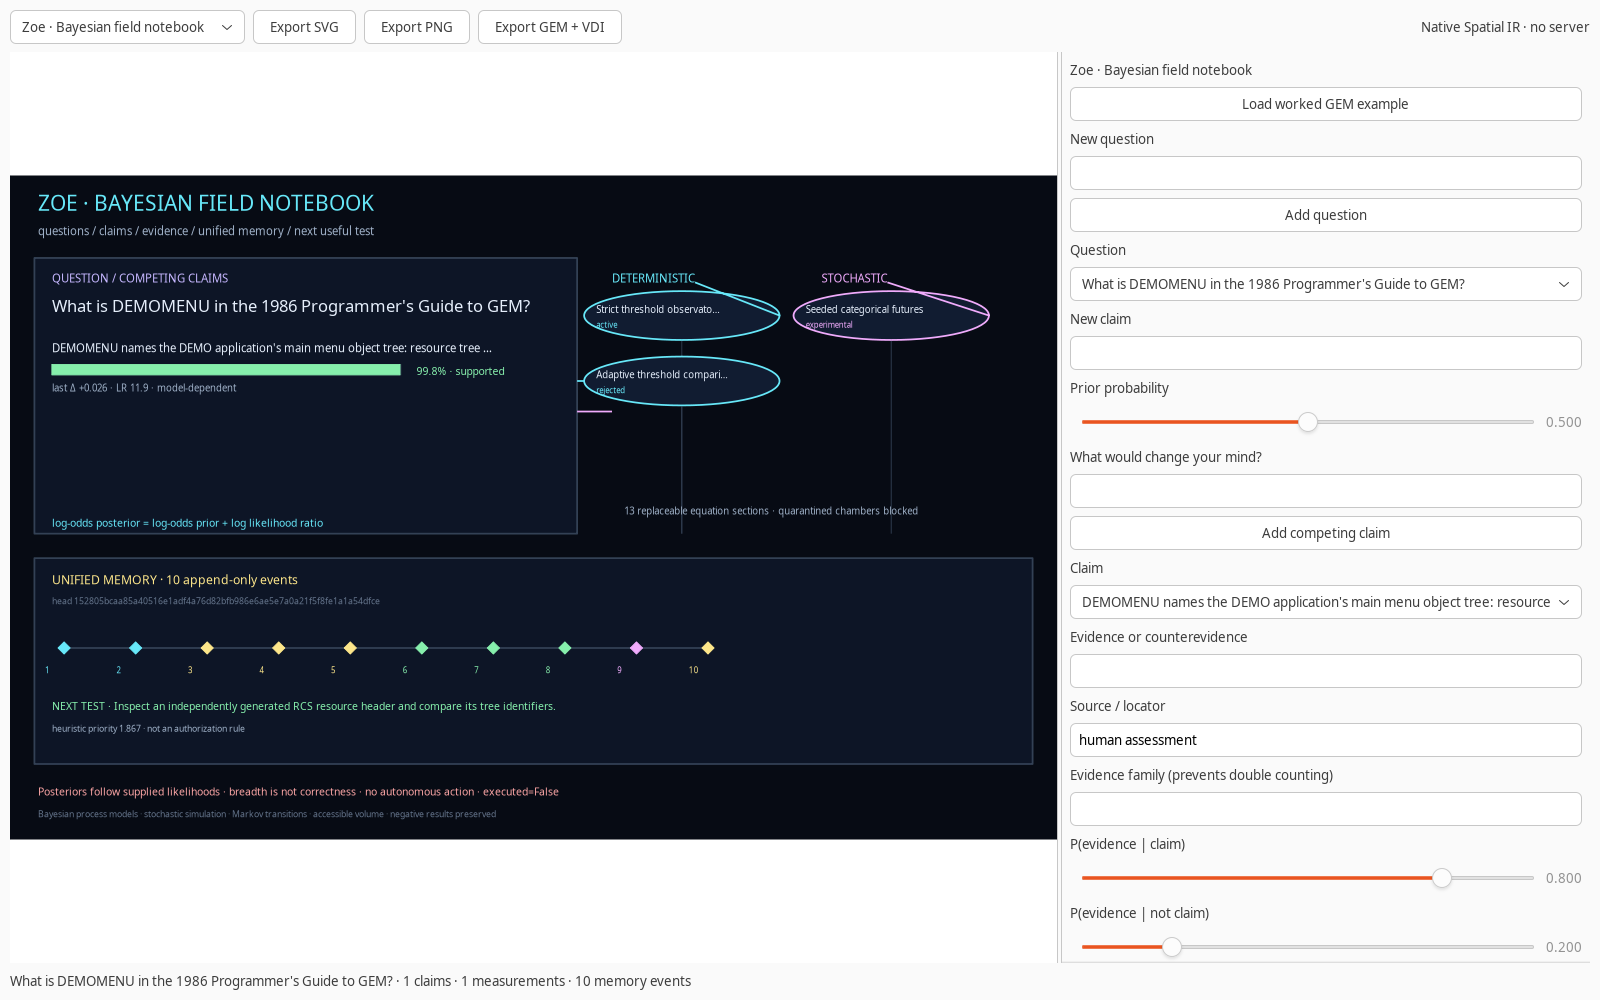
\includegraphics[width=\textwidth]{guiai-lab/docs/images/zoe-field-notebook.png}
\caption{A real notebook in Zoe: posterior bars, chamber states, the event-memory chain, and a next-test recommendation.}
\end{figure}

\section{Why this can matter}
\subsection{For artists and designers}
Zoe turns mathematical structure into something you can touch. You can make a shape, test a transformation, keep the evidence, and turn it into a poster or a native GEM metafile. The creative process remains inspectable rather than mysterious.

\subsection{For researchers}
Zoe is a place to keep competing explanations honest. You can preserve negative results, compare forecasts, and choose the next experiment without losing why you chose it. This is useful whenever confidence and evidence are not the same thing.

\subsection{For biology, genetics, and brain research}
A future notebook could hold genetic hypotheses, phenotype evidence, neural timing data, or competing models of a biological process. Zoe could help organize uncertainty and select the next measurement. These are future workflows to validate, not existing medical or neuroscientific capabilities. Zoe does not map the human brain, diagnose disease, or establish biological truth.

\subsection{For people who need evidence they can check}
A report is easier to trust when you can inspect the source, the event chain, and the reason for each change. Zoe's memory is append-only and hash-chained, so edits and reordering are visible. That is tamper evidence, not proof of identity or a substitute for good review.

\section{What was actually verified}
\begin{table}[htbp]
\centering
\caption{Verification you can repeat.}
\begin{tabular}{p{4.5cm}p{8cm}}
\toprule
Check & Result \\
\midrule
Zoe native tests & 25 passed under X11. \\
Zoe headless tests & 21 passed; 4 native-only skips (25 total). \\
Broader GEM tests & 20 passed under X11. \\
Standalone BRAIN GEM & 13 passed; 3 native-only skips (16 total). \\
Accessible Q-Volume & Threshold changes $-1$ and $+3$; labeled sweeps, finite approximation, and two-way JSON passed. \\
Research conformance & 17 checks passed. \\
Original model evidence & 16 model cases and 120 BioBERT cases independently recomputed. \\
Cerotto & 64 normal and 64 sanitizer tests passed; one EWF-dependent skip in each suite. \\
PALA & 25 Rust tests and 125 integration checks passed, with 2 optional skips. \\
Browser and packaging & 23 particles, no external requests or browser errors; wheel and source distributions passed. \\
\bottomrule
\end{tabular}
\end{table}

Some neighboring GUIAI tests have unrelated investigation-CLI and layout failures. Cerotto's bridge was not separately revalidated as part of Zoe. These are stated limits, not hidden successes.

\section{Try it yourself}
From the Zoe checkout:
\begin{lstlisting}
export MASTER_GEM_RESEARCH_ROOT=/path/to/next-token-predictability
PYTHONPATH=guiai-lab python -m guiai.gem zoe
PYTHONPATH=guiai-lab python -m guiai.gem zoe --module field
PYTHONPATH=guiai-lab python -m guiai.gem notebook --output zoe-field.json
PYTHONPATH=guiai-lab python -m guiai.gem notebook zoe-field.json --output zoe-field.svg
PYTHONPATH=guiai-lab python -m guiai.gem qualia --output accessible-q-volume.json
\end{lstlisting}
For the standalone notebook:
\begin{lstlisting}
python -m pip install /path/to/brain-gem
brain-gem field
brain-gem notebook --output field-memory.json
brain-gem notebook field-memory.json --output field-memory.svg
\end{lstlisting}
The demo memory, verification summary, source code, and visual evidence are embedded in the PDF. The 98 MB Groove probability archive stays in the next-token-predictability repository and is identified by SHA-256 rather than embedded.

\section{What Zoe does not do}
\begin{itemize}[nosep]
  \item It does not claim consciousness, sentience, or personhood.
  \item It does not guarantee future tokens, musical outcomes, correct beliefs, or good decisions.
  \item It does not diagnose patients, map the brain, or validate biological or genetic claims.
  \item It does not treat a sampled outcome as proof or a high-volume forecast as safe.
  \item Accessible Q-Volume annotates explicit causal repertoires. It does not replace $\Phi$ or $\gamma$, infer a causal model from a forecast, or turn a finite threshold sweep into an exact reconstruction.
  \item It does not execute recommendations automatically. The user decides.
  \item It does not replace source review, clinical validation, forensic custody, or human judgment.
\end{itemize}

\section{The fun part}
Zoe lets you ask a question and see the shape of the possible answers. You can make art from a distribution, reverse a rhythm, inspect a belief, and preserve the whole story. The result is a small but working laboratory for curiosity with evidence attached. That is the part worth sharing.

\appendix
\enlargethispage{2\baselineskip}
\section{Evidence and attachments}
This PDF embeds both paper sources, demo memory, the verification summary and conformance report, native screenshots, and five mechanism diagrams. Nicholas Michael Kloster solely created accessible volume on March 6, 2026. Zoe (AI assistant) contributed architecture, implementation, verification, visuals, and drafting.

\embedfile{paper/zoe-for-everyone.tex}
\embedfile{paper/zoe.tex}
\embedfile{paper/zoe-field-demo.json}
\embedfile{paper/verification-summary.json}
\embedfile{evidence/master-gem/conformance.json}
\embedfile{guiai-lab/docs/QUALIA.md}
\embedfile{guiai-lab/guiai/gem/qualia.py}
\embedfile{guiai-lab/docs/images/zoe-qualia.png}
\embedfile{evidence/qualia/accessible-q-volume.json}
\embedfile{guiai-lab/docs/images/zoe-visuals/01-epistemic-firewall.png}
\embedfile{guiai-lab/docs/images/zoe-visuals/02-belief-diff.png}
\embedfile{guiai-lab/docs/images/zoe-visuals/03-chambers.png}
\embedfile{guiai-lab/docs/images/zoe-visuals/04-memory-chain.png}
\embedfile{guiai-lab/docs/images/zoe-visuals/05-next-test.png}
\embedfile{guiai-lab/docs/images/zoe-brain.png}
\embedfile{guiai-lab/docs/images/zoe-field-notebook.png}
\embedfile{guiai-lab/docs/images/zoe-research.png}
\embedfile{guiai-lab/docs/images/cerotto-gem.png}

\end{document}
